\documentclass[12pt, twoside, a4paper]{report}
\author{Mayank Jatav}

%%%%%%%%%%%%%%%%%%%%%%%%%%%%%%%%%%%%%%%%%%%%%%%%%%%%%%%%%%%%%%%%%%%%%%%%%%%%%%%%%%%%%%%%%%%%%%%%%%%%%%

% Font Options
% Times New Roman and DropCap
\usepackage{mathptmx, lettrine}
\usepackage{mathtools,amsmath}
\usepackage{gensymb}
\usepackage{amsfonts}
\usepackage[useregional]{datetime2}
% Beautiful Math Font
\usepackage{eulervm}
\usepackage{pdfpages}

% Table Options
\usepackage{array, longtable, subcaption, multirow, tabularx, booktabs}
\captionsetup{%
	figurename=Figure,
	tablename=Table
}

% Graphics and Figure Options
\usepackage{graphics, float, xcolor}

% Aligning/Formatting Equations
\usepackage{amsmath}

% Typeset Text
\usepackage{microtype}
\usepackage{epstopdf}
\usepackage{subcaption}
\usepackage{graphicx}
\usepackage{tabularray}
\usepackage[normalem]{ulem}

% Customize Lists
\usepackage{enumitem}
\usepackage{lscape, rotating, layout}
\usepackage[a4paper, left=20mm, right=20mm, top=30mm, bottom=30mm]{geometry}	% Online

% Fancy Header
\usepackage{fancyhdr}
\fancyhf{}
\pagestyle{fancy}
\renewcommand{\headrulewidth}{0.4pt}
\renewcommand{\footrulewidth}{0.4pt}
\setlength{\headheight}{15pt}
\setlength{\footskip}{10mm}

% Referencing Options
\usepackage[numbers,sort&compress]{natbib} % Use natbib only, with numeric style

% Blank Pages - Empty Header
\usepackage{emptypage}
% Chapter Title Design
\usepackage[T1]{fontenc}
\usepackage[charter]{quotchap}

% Hyphenation
\usepackage{hyphenat}
\usepackage[english]{babel}
% Roman numbers
\usepackage{romannum}

% Number Formatter
\usepackage{siunitx}

% Color HyperLinks
\definecolor{darkpastelgreen}{rgb}{0.01, 0.75, 0.24}
\usepackage{hyperref, url}

% Online
\hypersetup{colorlinks=false, linkcolor=black, citecolor=darkpastelgreen, filecolor=magenta, urlcolor=blue}

% Acronyms/Glossary
\usepackage[nopostdot, style=super, nonumberlist, toc, automake, acronym]{glossaries}
\makeglossaries

\usepackage{adjustbox}

\renewcommand{\glsnamefont}[1]{\textbf{#1}}
\newacronym{ref}{ref}{Reference}
\newacronym{CNN}{CNN}{Convolutional Neural Network}
\newacronym{ViT}{ViT}{Vision Transformer}

% Macro commands
%%% keywords
\providecommand{\keywords}[1]{\textbf{\textit{Keywords---}} #1}
%%% Big O notation
\newcommand{\bigO}[1]{\ensuremath{\mathop{}\mathopen{}\mathcal{O}\mathopen{}\left(#1\right)}}

%%%%%%%%%%%%%%%%%%%%%%%%%%%%%%%%%%%%%%%%%%%%%%%%%%%%%%%%%%%%%%%%%%%%%%%%%%%%%%%%%%%%%%%%
\parskip 2.5mm		% Space before a New Paragraph
\parindent 0pt		% Indent Paragraphs
\linespread{1.3}	% Space between Lines of the paragraph

% Initialize Table of Contents, List of Figures and List of Tables
\AtBeginDocument{\addtocontents{toc}{\protect\thispagestyle{empty}}}
\AtBeginDocument{\addtocontents{lof}{\protect\thispagestyle{empty}}}
\AtBeginDocument{\addtocontents{lot}{\protect\thispagestyle{empty}}}
%%%%%%%%%%%%%%%%%%%%%%%%%%%%%%%%%%%%%%%%%%%%%%%%%%%%%%%%%%%%%%%%%%%%%%%%%%%%%%%%%%%%%%%%

\begin{document}

\pagenumbering{gobble}

% Title Page

\begin{titlepage}
\thispagestyle{empty}

%%%%%%%%%%%%%%%%%%%%%%%%%%%%%%%%%%%%%%%%%%%%%%%%%%%%%%%%%%%%%%%%%%%%%%%%%%%%%%%%%%%%%%%%%%%%%%%%%%%%%%

\begin{table}
	\centering
	\begin{tabular}{c}
		\Large \textbf{<<Title Here>>} \\
		\\
		\\
		\it Submitted in partial fulfilment of the requirements for the degree of	\\
		\bf Master of Technology	\\
		\\
		\\
		\\
		\it by	\\
		\large \bf {<<Name>>}	\\
		(Roll No. $<<roll no>>$)	\\
		\\
		\\
		\\
		\it under the supervision of	\\
		\large \bf <<Supervisor Name>>	\\

		\\
		\\
		\\
		\\
		
\includegraphics[width=.17\textwidth]{images/iiitdmj.png}	\\
		\\
		\normalsize{\textbf{Computer Science and Engineering}}	\\
		\\
		\bf PDPM INDIAN INSTITUTE OF INFORMATION TECHNOLOGY,	\\
		\bf DESIGN AND MANUFACTURING, JABALPUR	\\
		\bf INDIA	\\
		\\
		$\mathbf{<<year>>}$	\\
	\end{tabular}
\end{table}
\pagebreak

%%%%%%%%%%%%%%%%%%%%%%%%%%%%%%%%%%%%%%%%%%%%%%%%%%%%%%%%%%%%%%%%%%%%%%%%%%%%%%%%%%%%%%%%%%%%%%%%%%%%%%

\thispagestyle{empty}
\end{titlepage}

%%%%%%%%%%%%%%%%%%%%%%%%%%%%%%%%%%%%%%%%%%%%%%%%%%%%%%%%%%%%%%%%%%%%%%%%%%%%%%%%%%%%%%%%%%%%%%%%%%%%%%

\thispagestyle{empty}
% \null\vfill

\vspace*{6.5cm}
 \begin{center}
 \textbf{{{\LARGE{Dedicated to...}}}}\\
 \large{My Family }
 \end{center}
 %\vfill\null
 

%%%%%%%%%%%%%%%%%%%%%%%%%%%%%%%%%%%%%%%%%%
% Change Page Numbering Format
\pagenumbering{roman}

% Approval Sheet

% \chapter*{\center Approval Sheet}
\chapter*{Approval Sheet}
\thispagestyle{empty}

%%%%%%%%%%%%%%%%%%%%%%%%%%%%%%%%%%%%%%%%%%%%%%%%%%%%%%%%%%%%%%%%%%%%%%%%%%%%%%%%%%%%%%%%%%%%%%%%%%%%%%

\nohyphens{The thesis entitled \textbf{``Fabrics Classification using Deep Learning, Security Orchestration Automation and Response''} submitted by \textbf{Mayank Jatav} (Roll No. $23MCSA05$) is approved for partial fulfilment of the requirements for the degree of {\it \bf Master of Technology} in {\it \bf Computer Science and Engineering}.}

%%%%%%%%%%%%%%%%%%%%%%%%%%%%%%%%%%%%%%%%%%%%%%%%%%%%%%%%%%%%%%%%%%%%%%%%%%%%%%%%%%%%%%%%%%%%%%%%%%%%%%

\begin{table}[ht]
	\begin{tabular*}{\textwidth}{ l @{\extracolsep{\fill}} r }

		& \\
		& \\
		& \\
		& Examining Committee \\
		& \\
		& ................................................ \\
		& ................................................ \\
		& ................................................ \\

		& \\
		& Guide \\
		& \\
		& ................................................ \\
		& ................................................ \\
		& ................................................ \\
		&\\
		& Chairperson \\
		& \\
		& ................................................ \\

		Date: ..............................
		& ................................................ \\

		Place: Jabalpur
		& ................................................ \\

		& \\

	\end{tabular*}
\end{table}

%%%%%%%%%%%%%%%%%%%%%%%%%%%%%%%%%%%%%%%%%%%%%%%%%%%%%%%%%%%%%%%%%%%%%%%%%%%%%%%%%%%%%%%%%%%%%%%%%%%%%%

% Declaration

% \chapter*{\center Declaration}
\chapter*{Declaration}
\thispagestyle{empty}

%%%%%%%%%%%%%%%%%%%%%%%%%%%%%%%%%%%%%%%%%%%%%%%%%%%%%%%%%%%%%%%%%%%%%%%%%%%%%%%%%%%%%%%%%%%%%%%%%%%%%%

\vspace{1cm}
\nohyphens{I hereby declare that the submitted thesis entitled "<<Thesis Title>>" is my own work, and the work done by the undersigned has not been submitted anywhere for the award of any other degree or diploma in any university or other institutes of higher learning. All sources of information used in the current work have been duly acknowledged.
}

%%%%%%%%%%%%%%%%%%%%%%%%%%%%%%%%%%%%%%%%%%%%%%%%%%%%%%%%%%%%%%%%%%%%%%%%%%%%%%%%%%%%%%%%%%%%%%%%%%%%%%

\vspace*{3cm}
\begin{flushright}
    
	<<Name>>	\\
	\vspace*{0.2cm}
        Roll No. <<roll no>>\\
	 Date: ............................

\end{flushright}

%%%%%%%%%%%%%%%%%%%%%%%%%%%%%%%%%%%%%%%%%%%%%%%%%%%%%%%%%%%%%%%%%%%%%%%%%%%%%%%%%%%%%%%%%%%%%%%%%%%%%%

% Certificate

% \chapter*{\center Certificate}
\chapter*{Certificate}
\thispagestyle{empty}


%%%%%%%%%%%%%%%%%%%%%%%%%%%%%%%%%%%%%%%%%%%%%%%%%%%%%%%%%%%%%%%%%%%%%%%%%%%%%%%%%%%%%%%%%%%%%%%%%%%%%%

\nohyphens{This is to certify that the work contained in the thesis entitled \textbf{\textquotedblleft <<Thesis Title>> \textquotedblright} submitted by \textbf{<<Name>> (Roll No. <<roll no>>)} in partial fulfilment of the requirements for the degree of Master of Technology in Computer Science and Engineering has been carried out under my supervision and that this work has not been submitted elsewhere for the award of any other degree.}

%%%%%%%%%%%%%%%%%%%%%%%%%%%%%%%%%%%%%%%%%%%%%%%%%%%%%%%%%%%%%%%%%%%%%%%%%%%%%%%%%%%%%%%%%%%%%%%%%%%%%%

\begin{table}[ht]
	\begin{tabular*}{\textwidth}{l @{\extracolsep{\fill}} r }
		&	\\
		&	\\
		&	\\
		&	\\
		&	\\
		&	\\
		& \bf <<Supervisor Name>>	\\
		& Computer Science and Engineering Discipline	\\
		& PDPM Indian Institute of Information Technology,\\
            & Design and Manufacturing, Jabalpur	\\
		& India - $482005$ \\
		& Date: ........................ \\

	\end{tabular*}
\end{table}

%%%%%%%%%%%%%%%%%%%%%%%%%%%%%%%%%%%%%%%%%%%%%%%%%%%%%%%%%%%%%%%%%%%%%%%%%%%%%%%%%%%%%%%%%%%%%%%%%%%%%%


\chapter*{Acknowledgement}

Throughout the course of my Master's journey, I have been fortunate to receive guidance, encouragement, and support from several individuals, without whom this thesis would not have been possible. I take this opportunity to express my heartfelt gratitude to all those who have been an integral part of this academic endeavor.

First and foremost, I would like to express my deepest gratitude to my supervisor, \textbf{Prof. Pritee Khanna}, for her constant support, mentorship, and insightful guidance throughout the course of this work. Her expertise, constructive feedback, and patient encouragement have played a vital role in shaping the direction and quality of this research. I am also sincerely thankful to \textbf{Prof. Aparajita Ojha} for her consistent guidance and valuable suggestions. Her support, both academically and personally, helped me maintain a strong foundation throughout the research process.

I would like to extend my sincere thanks to my internship mentor, \textbf{Mr. Gaurav Damri}, for his mentorship, technical guidance, and for providing me the opportunity to work on real-world problems as part of my internship at Bharat Electronics Limited.

I am also thankful to my thesis committee members—\textbf{Dr. Avinash Chandra Pandey}, \textbf{Dr. Shivansh Mishra}, and \textbf{Dr. Nitish Andola}—for their time, insights, and constructive feedback which greatly helped in improving the quality of this work.

Beyond academic support, this journey was made easier and more fulfilling thanks to the unwavering encouragement and companionship of my peers. I would like to express heartfelt appreciation to \textit{Mohammad Arif Khan}, \textit{Amit Bhati}, \textit{Poornima Singh Thakur}, \textit{Shubhangi Chaturvedi}, \textit{Janvi Gohil}, \textit{Sudha Singh}, and \textit{Aman Yerwarkar} for their constant moral support, discussions, and uplifting presence.

Lastly, I owe my deepest gratitude to my family, for their unconditional love, sacrifices, and support throughout my life. Their faith in me has been my greatest strength.

\bigskip

\hfill\textit{--- Mayank Jatav}

% Abstract

% \chapter*{\center Abstract}
\chapter*{Abstract}
\pagestyle{plain}
\thispagestyle{empty}

%%%%%%%%%%%%%%%%%%%%%%%%%%%%%%%%%%%%%%%%%%%%%%%%%%%%%%%%%%%%%%%%%%%%%%%%%%%%%%%%%%%%%%%%%%%%%%%%%%%%%%
%%%%%%%%%%%%%%%%%%%%%%%%%%%%%%%%%%%%%%%%%%%%%%%%%%%%%%%%%%%%%%%%%%%%%%%%%%%%%%%%%%%%%%%%%%%%%%%%%%%%%%
%%%%%%%%%%%%%%%%%%%%%%%%%%%%%%%%%%%%%%%%%%%%%%%%%%%%%%%%%%%%%%%%%%%%%%%%%%%%%%%%%%%%%%%%%%%%%%%%%%%%%%

Write abstract here ..............

%%%%%%%%%%%%%%%%%%%%%%%%%%%%%%%%%%%%%%%%%%%%%%%%%%%%%%%%%%%%%%%%%%%%%%%%%%%%%%%%%%%%%%%%%%%%%%%%%%%%%%
%%%%%%%%%%%%%%%%%%%%%%%%%%%%%%%%%%%%%%%%%%%%%%%%%%%%%%%%%%%%%%%%%%%%%%%%%%%%%%%%%%%%%%%%%%%%%%%%%%%%%%
%%%%%%%%%%%%%%%%%%%%%%%%%%%%%%%%%%%%%%%%%%%%%%%%%%%%%%%%%%%%%%%%%%%%%%%%%%%%%%%%%%%%%%%%%%%%%%%%%%%%%%
\vspace{0.4cm}
\keywords{Add keyword here seperated by ','}
%%%%%%%%%%%%%%%%%%%%%%%%%%%%%%%%%%%%%%%%%%%%%%%%%%%%%%%%%%%%%%%%%%%%%%%%%%%%%%%%%%%%%%%%%%%%%%%%%%%%%%
%%%%%%%%%%%%%%%%%%%%%%%%%%%%%%%%%%%%%%%%%%%%%%%%%%%%%%%%%%%%%%%%%%%%%%%%%%%%%%%%%%%%%%%%%%%%%%%%%%%%%%
%%%%%%%%%%%%%%%%%%%%%%%%%%%%%%%%%%%%%%%%%%%%%%%%%%%%%%%%%%%%%%%%%%%%%%%%%%%%%%%%%%%%%%%%%%%%%%%%%%%%%%

\addcontentsline{toc}{chapter}{Abstract}

% Table of Contents and Lists
\setcounter{tocdepth}{5}
\tableofcontents

\phantomsection
% Abbreviations

% \chapter*{\center Abbreviations}
\chapter*{Abbreviations}
\pagestyle{plain}
\thispagestyle{empty}

%%%%%%%%%%%%%%%%%%%%%%%%%%%%%%%%%%%%%%%%%%%%%%%%%%%%%%%%%%%%%%%%%%%%%%%%%%%%%%%%%%%%%%%%%%%%%%%%%%%%%%

\renewcommand{\glossarysection}[2][]{}
\printglossary[type=\acronymtype, style=listdotted]

%%%%%%%%%%%%%%%%%%%%%%%%%%%%%%%%%%%%%%%%%%%%%%%%%%%%%%%%%%%%%%%%%%%%%%%%%%%%%%%%%%%%%%%%%%%%%%%%%%%%%%
%%%%%%%%%%%%%%%%%%%%%%%%%%%%%%%%%%%%%%%%%%%%%%%%%%%%%%%%%%%%%%%%%%%%%%%%%%%%%%%%%%%%%%%%%%%%%%%%%%%%%%
%%%%%%%%%%%%%%%%%%%%%%%%%%%%%%%%%%%%%%%%%%%%%%%%%%%%%%%%%%%%%%%%%%%%%%%%%%%%%%%%%%%%%%%%%%%%%%%%%%%%%%

\addcontentsline{toc}{chapter}{List of Abbreviations}

\listoffigures
\addcontentsline{toc}{chapter}{List of Figures}

\listoftables
\addcontentsline{toc}{chapter}{List of Tables}

%%%%%%%%%%%%%%%%%%%%%%%%%%%%%%%%%%%%%%%%%%
\renewcommand{\sectionmark}[1]{\markright{\thesection\ #1}}

\setcounter{page}{1}
\pagenumbering{arabic}

%%%% Chapters %%%%%%
% PART I: Research Work
\chapter{Introduction}

As a part of my Master’s program, I had the opportunity to work on two very different but equally valuable projects—one in research and the other in a practical, industry-based environment. This thesis brings together both experiences in a single document. The first part describes a research project I worked on about the topic Fabric classification using deep learning, and the second part focuses on my internship work in the field of Security Orchestration, Automation, and Response (SOAR).

Both projects helped me to step out of my comfort zone and exposed me to different aspects of the tech world. The research work taught me how to approach technical problems from a scientific perspective that included reading papers, building models, analyzing results—all while diving deep into machine learning. On the other hand, my internship was much more hands-on, where I got a change to be part of a team developing a cybersecurity tool. This involved writing code for both the backend and frontend, working with APIs, and figuring out how everything ties together in a real world software system.

These experiences were not just about learning new tools or technologies but they also gave me a clear understanding of how AI is being used to solve real problems, whether it’s about predicting threat responses or identifying fabric types using images. I also learned a lot from the people I worked with, who shared their own knowledge and helped me think more critically and practically about building solutions.

\section{Research Work - Fabric Classification using Deep Learning}
% Briefly introduce your research work here.

My research project focused on \textbf{fabric classification using deep learning}, a critical application within computer vision and artificial intelligence. The objective was to develop an automated system capable of accurately identifying different types of fabrics from images. This problem holds significant relevance in various industries, including textile manufacturing, fashion retail, and quality control, where manual classification is often time-consuming, prone to human error, and lacks scalability.

My work involved a comprehensive exploration of deep learning techniques, specifically \textbf{convolutional neural networks (CNNs)} and \textbf{Vision Transformers}, which are exceptionally well-suited for image-based recognition tasks. The research process encompassed several key stages:
\begin{itemize}
    \item \textbf{Literature Review and Implementation}: I began by delving into existing research, specifically implementing and analyzing three prominent papers in the field:
    \begin{enumerate}
        \item ``\textbf{Research on Classification of Clothing Fabrics Images Based on Convolutional Neural Network}'' This paper provided foundational insights into using CNNs for fabric classification.
        \item ``\textbf{TextileNet: A Deep Learning Approach for Textile Fabric Material Identification from OCT and Macro Images}'' This work expanded my understanding of employing deep learning for textile material identification across different image modalities.
        \item ``\textbf{Fabric Composition Identification using Fine-Tuned Vision Transformers}'' This research introduced me to the advanced capabilities of Vision Transformers in fine-grained image classification tasks, which proved invaluable for identifying fabric compositions.
    \end{enumerate}
    \item \textbf{Data Collection and Preprocessing}: Following the insights gained from these implementations, I curated and prepared a diverse dataset of fabric images, addressing challenges such as varying lighting conditions, textures, and image resolutions to ensure robust model training.
    \item \textbf{Model Development and Training}: Beyond replicating existing models, I then proceeded to build and implement my own deep learning model for fabric classification. This involved designing a custom architecture, experimenting with different configurations, and performing extensive hyperparameter tuning to optimize performance.
    \item \textbf{Performance Evaluation}: I rigorously assessed both the implemented models from the literature and my custom-built model's accuracy, precision, recall, and F1-score to determine their effectiveness in classifying various fabric types. A comparative analysis highlighted the strengths and weaknesses of each approach, demonstrating the efficacy of my proposed solution.
\end{itemize}
This research not only provided practical insights into applying deep learning for image classification but also significantly enhanced my understanding of scientific methodology, including comprehensive literature review, experimental design, model development, and critical analysis of results. The findings from this project culminated in a publication, demonstrating its contribution to the academic discourse.

\section{BEL Internship - Security, Orchestration, Automation and Response}
My internship at Bharat Electronics Limited (BEL) provided an invaluable opportunity to engage with the practical aspects of cybersecurity, specifically in the domain of \textbf{Security, Orchestration, Automation, and Response (SOAR)}. In today's complex threat landscape, Security Operations Centers (SOCs) face an overwhelming volume of alerts and incidents, making manual response impractical and inefficient. SOAR platforms are designed to address these challenges by integrating security tools, automating routine tasks, and orchestrating complex incident response workflows.

During my internship, I was an integral part of a team developing a SOAR solution aimed at enhancing the efficiency and effectiveness of threat detection and response within a real-world operational environment. My contributions involved:
\begin{itemize}
    \item \textbf{Backend Development}: Implementing robust backend logic to process security alerts, integrate with various security tools via APIs, and manage incident data. This included working with databases and designing efficient data pipelines.
    \item \textbf{Frontend Development}: Creation of a user-friendly web interface for the SOAR platform, enabling security analysts to visualize alerts, manage incidents, and execute automated response actions.
    \item \textbf{AI Model Integration}: Developing a machine learning model capable of understanding natural-language descriptions of incidents and recommending action to mitigate the incident. This included dataset preparation, model training, evaluation, and integration with the SOAR backend.
\end{itemize}
This hands-on experience provided me with a deep understanding of the practical challenges in cybersecurity operations and the critical role of automation in mitigating risks. It also honed my skills in full-stack development, collaborative software engineering, and problem-solving within a dynamic industry setting. The successful completion of this internship is marked by an official certificate from Bharat Electronics Limited.
\chapter{Fabric Classification using Deep Learning}

Textiles can be found globally across many industries—not only apparel and fashion, but also in home furnishings, healthcare, automotive and aerospace industries, etc. Each fabric exhibits a unique texture, appearance, and structure. There are over 25,000 fabric types, and successfully identifying the fabrics can be challenging. Fabric identification is important because the fabric type typically dictates what the fabric is suitable for e.g., garments (apparel), medical (medical supplies), and interior (furnishings). 

In the past, fabrics were exclusively identified by manual and chemical means, which included burn tests, solubility tests, and microscopic examination of fibers. Although the manual and chemical methods can be useful, they can be time-consuming and require proficient practitioners. With industries that require quick decisions or involve large-scale processing, such as fast fashion or textile manufacturing, the manual identification approaches are not always suitable.

Recent advances in computer vision and deep learning open up new possibilities for fabric classification automation, and deep learning models can learn fine-grained patterns and textures through images, therefore enabling reliable model fabric classification without handcrafted features; additionally, vision transformers (ViTs) have become robust models able to model global relationships in images, therefore ViT models may be able to model complex texture and structure for fabric. 

In this chapter, we compare deep learning methods of classifying fabrics with images. The first method is based on transfer learning using a VGG-16 model from a set of fabric images. In the second method, TextileNet, we compare multiple pre-trained CNN models from two datasets: Optical Coherence Tomography (OCT) fabric images and macro fabric images. We have illustrated the comparably strong performance of MobileNetV2 when working with the OCT images and the third method is using a Vision Transformer as a feature extractor combined with PCA, LDA and a support vector machine (SVM) for classification scores.

By utilizing and analyzing these methods, we come to understand both the benefits and the limitations of the two methods of classification. Based on the insights of the two methods of classification, we propose a new model that combines a CNN branch and a Vision Transformer branch to improve the robustness and accuracy of fabric classification.

% Overview of the research project.
\section{Fibre and Fabric: Understanding the Distinction}

In textile production, both "fibre" and "fabric" terms are commonly used. Fibre and fabric are both related, but they represent different steps in the creation of textiles. Knowing the differences between fibres and fabrics is important to understand the basic mechanisms of the textile manufacturing process and the characteristics of the final product.

\subsection{Fibre}

A \textbf{fibre} is the most basic building block of any textile material. It is a thin, thread of filament or a natural or man-made substance that is much longer than it is width. These individual filaments incorporate the inherent attributes that characterize the textile. The principal function of fibres is to be spun into a yarn; that yarn is then used to produce fabric \cite{researchgate}.

\textbf{Key characteristics of fibres:}
\begin{itemize}
    \item \textbf{Fundamental Unit:} Fibres are the smallest and most elementary components from which textiles are formed.
    \item \textbf{Filamentary Structure:} They possess a slender, elongated, and thread-like shape.
    \item \textbf{Source:} Fibres can be natural (e.g., obtained from plants like cotton, linen, jute; from animals like wool, silk) or synthetic (e.g., polyester, nylon, acrylic) \cite{researchgate}.
    \item \textbf{Properties:} The properties of a fibre (e.g., strength, elasticity, absorbency, softness, insulation) is a direct extension of the properties of used fibres as they influence the properties of the yarn and final fabric \cite{researchgate}.
    \item \textbf{Not directly usable as clothing:}  Fibres are usually too fine and short (staple fibres, e.g., cotton) or too weak (continuous filaments, e.g., silk before twist) to use individually in the construction of garments or most textile products. Fibres must be processed into yarn before being used \cite{researchgate}.
\end{itemize}

\textbf{Examples of Fibres:}
\begin{itemize}[noitemsep, topsep=0pt]
    \item \textbf{Natural:} Cotton, Linen, Jute, Wool, Silk, Hemp.
    \item \textbf{Synthetic:} Polyester, Nylon, Rayon, Spandex (Lycra), Acrylic.
\end{itemize}

\subsection{Fabric}

A \textbf{fabric} is, on the other hand, the material derived from interlacing, looping or otherwise bonding fibres or yarns together. Fabric is a more dense and cohesive material and may be used directly with minimal processing to produce clothing, home furnishings, industrial products, and a wide range of textile-based types of goods. Fabric is the result of several processes that convert raw fibres or yarns to attached or laminated fibres or yarns in sheet form \cite{researchgate, hong2024research}.

\textbf{Key attributes of fabrics:}
\begin{itemize}
    \item \textbf{Constructed Material:} Fabrics are the assembled arrangement of fibres or more often yarns. 
    \item \textbf{Methods of Construction:} Some of the methods that are commonly employed for making textiles are: 
        \begin{itemize}
            \item \textbf{Weaving:} The process (warp and weft) of interlacing two systems of yaml at right angles to one another forming a stable structure.
            \item \textbf{Knitting:} The interlooping of a single type of yarn can produce a warm, flexible stretching-yarn material.
            \item \textbf{Felting:} A process that may employ heat, moisture and friction where the fibres (usually wool) are pressed and then matted together to bind them to produce a dense solid nonwoven textile material.
            \item \textbf{Non-woven:} A process that provides some type of bonding (chemical, mechanical or thermal) of fibres without going through a spinning operation or weaving/knitting operation \cite{hong2024research}.
        \end{itemize}
        \item \textbf{Directly Usable:} Fabrics are completed textile materials both cut, sewn or finished to use in garment or product production.
        \begin{figure}[H]
            \centering
            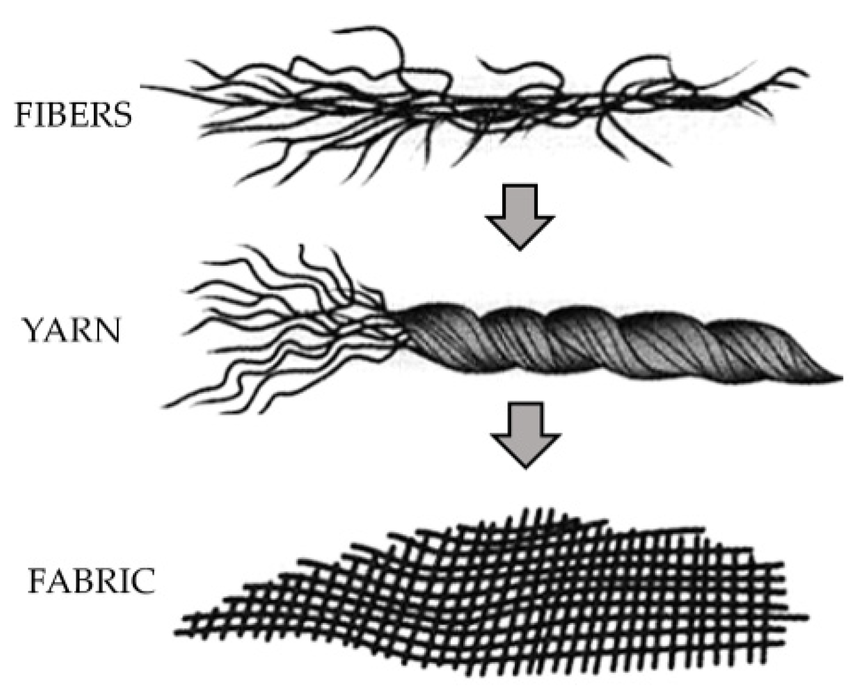
\includegraphics[width=0.6\textwidth]{images/fabric_construction}
            \caption{Construction of Fabric from Fibres}
            \label{fig:fabric_construction}
        \end{figure}
    \item \textbf{Properties derived from fibres and construction:} The properties of a fabric (e.g., drape, hand, durability, breathability, warmth) are determined by the fibres from which the yarn(s) are made, the fibres or yarns used, and the method used to construct the fabric (woven, knitted, etc.) \cite{researchgate, hong2024research}.
\end{itemize}

\textbf{Examples of Fabrics:}
\begin{itemize}[noitemsep, topsep=0pt]
    \item Cotton fabric, Silk fabric, Wool fabric, Polyester fabric, Denim, Chiffon, Fleece, Canvas.
\end{itemize}

\subsection{Differences between Fibre and Fabric}

It is necessary to remember that the textile industry is based upon the transformation process that connects fibre and fabric, to have context for the comparison. This transformation process takes raw materials through many different steps to turn them into functional and aesthetic products through a convoluted process of spinning, weaving, knitting, or bonding, etc. Designers, producers, and consumers must all acknowledge the fundamental connection between fibre and fabric, which demonstrates how raw materials are transformed into textiles we regularly use in our daily lives for apparel, furnishings, and other items. The table below segments their differences based on their roles and characteristics in textile processes.

\newpage

\begin{table}[h!]
    \centering
    \caption{Key differences between Fibre and Fabric}
    \label{tab:fibre_fabric_diff}
    \begin{tabular}{l p{5cm} p{5cm}} % Adjust column width for content
        \toprule
        \textbf{Feature} & \textbf{Fibre} & \textbf{Fabric} \\
        \midrule
        \textbf{Definition} & A single, thread-like filament or natural/synthetic substance \cite{researchgate}. & A material produced by weaving, knitting, felting, or bonding fibres/yarns \cite{researchgate, hong2024research}. \\
        \textbf{Form} & Basic, raw, individual component. & Constructed, cohesive, sheet-like material. \\
        \textbf{Stage of Production} & Precursor to yarn. The fundamental unit. & End product of textile formation (from yarn/fibre). \\
        \textbf{Usability} & Not directly used for clothing/products (must be processed) \cite{researchgate}. & Directly usable for making clothing and other textile products. \\
        \textbf{Properties} & Determines inherent characteristics (e.g., raw strength, absorbency) \cite{researchgate}. & Properties result from fibre type \textit{and} construction method (e.g., drape, texture, finished strength) \cite{researchgate, hong2024research}. \\
        \textbf{Analogy} & Think of individual strands of hair. & Think of a piece of cloth woven from those hair strands. \\
        \bottomrule
    \end{tabular}
\end{table}

In short, fibres are raw ingredients, fabrics are the cooked meal, ready to be consumed (or in this case, made into garments). The process from multiple single adjustments of fibres, to a usable, textured fabric, involves significantly complex processes which define the aesthetic, tactile, and functional qualities of the final textile product.
\section{Literature Review}

Fabric classification has been an area of growing interest in the fields of computer vision and material science due to its wide range of applications across industries such as fashion, healthcare, manufacturing, and forensics. With the advancement of deep learning, researchers have been exploring automated methods to accurately identify and classify textile materials using image data.

Traditionally, fabric classification relied on manual techniques and physical testing, but these approaches are time-consuming, prone to human error, and often require specialized equipment. In contrast, image-based classification using deep learning models offers a scalable and efficient alternative that can be used even in real-time applications.

In this section, we review key research contributions that have applied deep learning techniques for fabric classification. The datasets described here, used in these studies are carefully considered, as data quality and diversity are vital to achieving strong model performance. We also provide a detailed discussion of the three papers that were selected and implemented as part of this research work. Each paper highlights a different modeling approach offering valuable insights into the strengths and limitations of current methodologies.

By analyzing these works, we aim to identify the common practices, innovative ideas, and existing challenges in the domain, which in turn have shaped the direction of our proposed methodology.

\subsection{Dataset Overview}

The development of accurate and generalizable deep learning models for fabric classification is heavily dependent on the availability of high-quality, diverse, and well-structured datasets. Each dataset used in this domain captures textile properties from a unique perspective—some focus on fine surface-level textures, others provide microscopic or structural imaging, and some present large-scale image collections labeled through expert-driven taxonomies.

In this section, we present a detailed review of three key datasets that were used in the implementation and evaluation of deep learning models for this research. These datasets have been selected for their relevance, diversity, and their ability to represent different challenges in fabric classification. Each dataset has contributed to our understanding of how fabrics can be categorized based on visual cues, micro-structures, and material properties. The datasets reviewed are described below:

\newpage
\subsubsection{A. Fine-Grained Material Classification Using Micro-geometry and Reflectance~\cite{kampouris2016fine}}

One of the foundational datasets used for fine-grained material classification is based on micro-geometry and reflectance properties. This dataset, introduced by Kampouris et al., captures subtle material differences through high-resolution images that include shape, surface detail, and reflectance captured under varying lighting conditions.

The dataset was developed to aid in distinguishing materials that are visually similar to the human eye but differ in their physical or optical properties. It includes a range of fabrics and other material surfaces, photographed under controlled settings using a multi-light camera rig. Each sample is captured from multiple angles and under multiple lighting directions to collect reflectance fields. This setup allows for capturing texture, gloss, and geometric cues that are often difficult to extract from standard RGB images.

\begin{figure}[H]
    \centering
    \begin{minipage}{0.8\linewidth}
        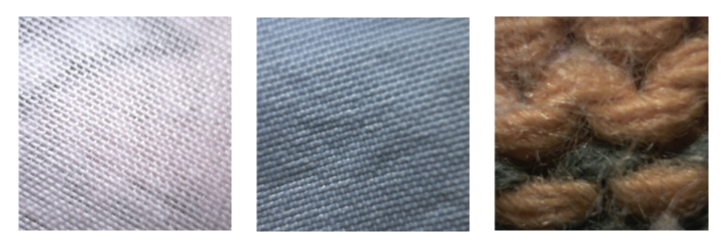
\includegraphics[width=\linewidth]{images/iBugDataset}
    \end{minipage}
    \caption[Sample images from the iBug Fabric Dataset]{Sample images from the iBug Fabric Dataset: (Left) Cotton, (Middle) Polyester, (Right) Wool.}
\end{figure}

What makes this dataset particularly useful for material classification is its emphasis on surface detail and reflectance behavior, rather than color or pattern alone. This makes it ideal for deep learning models that aim to identify materials based on physical characteristics, which are more consistent across environments compared to visual patterns.

Although the dataset covers a broader range of materials beyond textiles, its fabric subset is still highly valuable. It includes fabrics like cotton, wool, denim, and silk—each captured in fine detail—providing strong training data for distinguishing between these visually similar but structurally different materials.

This dataset serves as a strong foundation for deep learning models focused on material classification in fine-grained scenarios and is especially relevant when the goal is to distinguish fabrics based on their structural textures and reflectance rather than color or shape alone.

\subsubsection{B. Optical Coherence Tomography Image Dataset of Textile Fabrics~\cite{sabuncu2022optical}}

The Optical Coherence Tomography (OCT) image dataset of textile fabrics is a unique and specialized dataset that provides high-resolution cross-sectional images of fabric structures. Developed by Sabuncu and Ozdemir, this dataset aims to support material classification tasks through depth imaging and has proven useful for textile engineering, recycling, and forensic analysis.

The dataset includes OCT scans of fabrics made purely from cotton, wool, and polyester. For each material type, three different fabric samples were selected, resulting in a total of nine fabric categories. Using the Thorlabs CAL110C1 OCT system, each sample was scanned at over a hundred random surface locations to generate detailed cross-sectional images, commonly known as B-scans. The scan length was fixed at 2\,mm across all samples, and images were stored in raw \texttt{.png} format without any additional filtering or preprocessing.

\begin{figure}[H]
    \centering
    \begin{minipage}{0.8\linewidth}
        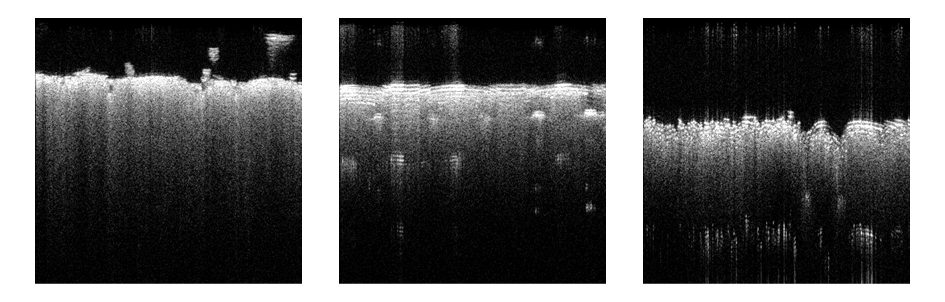
\includegraphics[width=\linewidth]{images/FabricOCTDataset.png}
    \end{minipage}
    \caption[Sample images from the Fabric OCT Dataset]{Sample images from the Fabric OCT Dataset: (Left) Cotton, (Middle) Polyester, (Right) Wool.}
\end{figure}

A key advantage of OCT imaging lies in its ability to reveal internal microstructural features of the fabric that are not visible in standard RGB images. These features include weave patterns, layer thickness, and material density, making OCT particularly valuable for classifying fabrics that may appear visually similar on the surface.

The dataset was structured into three main folders—cotton, wool, and polyester—each containing multiple scans from different fabric pieces of the same material. This setup provides a clean and well-labeled dataset that is suitable for training and testing deep learning models, especially those focused on learning from structural features rather than visual appearance alone.

Overall, the OCT image dataset offers a high degree of consistency and detail, which makes it ideal for tasks that require fine-grained classification of fabric types based on internal structure. Its application extends beyond classification, with potential uses in recycling processes, textile defect detection, and automated quality control in textile production.

\subsubsection{C. TextileNet: A Material Taxonomy-Based Fashion Textile Dataset~\cite{zhong2023textilenet}}

TextileNet is a large-scale, taxonomy-driven dataset designed to support textile material identification using deep learning techniques. Introduced by Shu Zhong et al., it addresses a major gap in existing datasets by providing a structured taxonomy of textile materials, divided into two primary categories: fibres and fabrics. Unlike most fashion-related datasets that often mix fibre and fabric labels or contain vague annotations, TextileNet provides a clearly defined and scientifically grounded label structure developed in collaboration with material science experts.

The dataset is split into two parts: \textit{TextileNet-fibre} and \textit{TextileNet-fabric}, comprising 33 fibre labels and 27 fabric labels, respectively. The total dataset consists of approximately 760,949 images, sourced from Google Images and reconstructed fashion datasets like iMaterialist. The image collection process was carefully curated using keyword-based queries derived from the defined textile taxonomies, ensuring that the dataset reflects real-world clothing items while maintaining a consistent label scheme.

\begin{figure}[H]
    \centering
    \begin{minipage}{0.8\linewidth}
        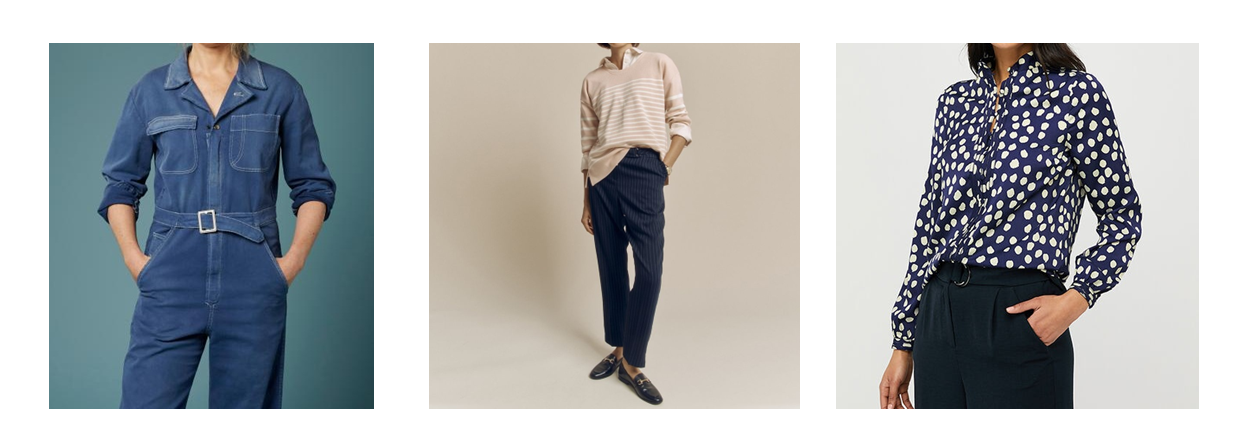
\includegraphics[width=\linewidth]{images/TextileNetDataset.png}
    \end{minipage}
    \caption[Sample images from the TextileNet Dataset]{Sample images from the TextileNet Dataset: (Left) Denim, (Middle) Crepe, (Right) Satin.}
\end{figure}

What makes TextileNet particularly valuable is its taxonomy-based design. The fibre taxonomy includes natural, synthetic, and regenerated fibres such as cotton, wool, polyester, bamboo viscose, and milk casein. The fabric taxonomy, on the other hand, categorizes textiles based on their production method (woven, knitted, non-woven) and includes examples like denim, tweed, velvet, and jersey.

% The dataset has been validated using both Convolutional Neural Networks (CNNs) and Vision Transformers (ViTs), with baseline models achieving over 80\% top-5 accuracy on classification tasks. It not only serves as a resource for textile classification but also supports sustainability-focused goals by enabling traceability of garments back to their fibre and fabric origins—a key step in promoting textile circularity.

Overall, TextileNet is suitable for training robust models that can identify complex fabric compositions in garments, supporting applications in retail, recycling, supply chain management, and sustainable fashion design.
\section{Methodology}

Recent advances in deep learning have significantly improved image-based classification tasks, particularly in domains involving fine-grained visual features such as textile analysis. In the context of fabric classification, challenges arise due to the high similarity between textile types (e.g., cotton vs. polyester), varying lighting conditions, and blended compositions. Existing methods based on Convolutional Neural Networks (CNNs) have shown notable success in capturing local textures and patterns in fabrics~\cite{hong2024research, kampouris2016fine}. However, CNNs often struggle to capture long-range dependencies or contextual information, which can be crucial for distinguishing between visually similar materials.

On the other hand, Vision Transformers (ViTs) have emerged as powerful models capable of modeling global relationships in image data through self-attention mechanisms~\cite{dosovitskiy2020vit}. Although ViTs have shown strong performance in general image recognition tasks, their effectiveness in fabric classification—especially for small datasets or subtle visual differences—has only recently been explored~\cite{chitra2023fabric}.

Motivated by the limitations and strengths of both approaches, this work proposes a hybrid deep learning architecture that integrates CNN and ViT components in a parallel configuration. The model is designed to harness the \textit{local feature extraction capabilities of CNNs} alongside the \textit{global context modeling of ViTs}, aiming to improve classification accuracy across different types of textile fabrics. The approach builds upon insights from \textit{TextileNet}, where multi-modal imaging (macro and OCT) was used to improve recognition of subtle structural differences in textiles~\cite{siam2023textilenet}.

This methodology section details the architecture of the proposed model, the role of each component, the strategy for feature fusion, and the final classification process. The design supports end-to-end training and is validated using well-structured fabric datasets.

\subsection{Convolutional Neural Networks (CNNs)}

Convolutional Neural Networks (CNNs) have become a cornerstone in the field of computer vision due to their effectiveness in automatically learning hierarchical feature representations from raw image data. Originally popularized for tasks such as handwritten digit recognition and object detection, CNNs have also proven highly effective in domains where texture, shape, and local patterns play a significant role—such as textile and fabric classification.

A CNN typically consists of a series of convolutional layers followed by non-linear activation functions (e.g., ReLU), pooling layers, and fully connected layers. The convolutional layers act as feature extractors, learning local filters that can detect edges, textures, and patterns at various levels of abstraction. As the network deepens, it builds increasingly complex and semantically rich representations, which are well-suited for distinguishing between different fabric types that may exhibit subtle differences in weave, fiber orientation, or surface reflectivity~\cite{simonyan2015vgg, lecun1998gradient}.

In this work, a CNN-based stream is designed as part of a hybrid model, consisting of four convolutional blocks with progressively increasing output channels (8, 16, 32, 64). Each block applies a $3\times3$ convolution operation with a stride of 3, followed by a ReLU activation. This architecture efficiently reduces the spatial resolution while preserving essential texture and pattern information—a technique previously shown to be effective in textile classification tasks~\cite{hong2024research}.

Studies such as by Kampouris et al.~\cite{kampouris2016fine} and Hong et al.~\cite{hong2024research} have demonstrated the success of CNNs in classifying fabric materials based on surface and structural characteristics. Furthermore, in practical applications, CNNs have been favored for their ability to generalize well to real-world textile images, including those captured under varying lighting conditions and camera settings.

While CNNs are powerful in learning local features, they are inherently limited in capturing global dependencies across spatial regions, which may affect performance when dealing with patterned fabrics. To address this limitation, CNNs are combined in this study with Vision Transformer (ViT) encoders, described in the following section, to capture both local and global representations of fabric structures.

\subsection{Vision Transformers (ViTs)}

Vision Transformers (ViTs) have emerged as a powerful alternative to convolutional architectures for image classification tasks. Unlike Convolutional Neural Networks (CNNs), which operate on local receptive fields, ViTs leverage self-attention mechanisms to model global relationships between different parts of an image. This makes them particularly suitable for applications like fabric classification, where understanding the spatial layout and contextual relationships between texture patterns is important~\cite{dosovitskiy2020vit}.

A standard Vision Transformer operates by first dividing an image into fixed-size patches (e.g., $16 \times 16$ pixels), which are flattened and projected into a latent embedding space using a linear layer. These patch embeddings, along with a learnable class token and positional encodings, are passed into a stack of Transformer encoder layers. Each encoder layer consists of two main subcomponents:
\begin{itemize}
    \item \textbf{Multi-Head Self-Attention (MHSA):} Computes pairwise attention scores between patches, enabling the model to capture long-range dependencies.
    \item \textbf{Feed-Forward Network (FFN):} A two-layer fully connected network with non-linearity (typically GELU), applied independently to each patch embedding.
\end{itemize}

Layer normalization and residual connections are applied around both subcomponents to enhance training stability. The final output corresponding to the class token is used for classification purposes.

In this study, the ViT branch consists of four sequential Transformer encoder layers, each of which processes the patch embeddings generated from the input image. The aim is to extract \textit{global and contextual features} that are particularly useful when dealing with fabrics that contain repeating patterns, folds, or blended fibers, where large-scale spatial context contributes to accurate classification~\cite{chitra2023fabric, siam2023textilenet}.

While CNNs are inherently biased toward local feature extraction, ViTs offer greater flexibility by modeling relationships across the entire image without positional locality assumptions. This property makes them highly effective in fabric classification scenarios, where a fiber's spatial structure can influence its identification. Moreover, recent research shows that ViTs can outperform CNNs when trained on sufficiently large datasets or when used in hybrid systems~\cite{dosovitskiy2020vit, touvron2021training}.

By integrating a ViT stream in parallel with a CNN stream, this work aims to build a hybrid system capable of leveraging both local textures and global structure, resulting in a more robust and accurate fabric classification model.

\subsection{Feature Fusion and Classification}

Once the image has been processed independently by the Convolutional Neural Network (CNN) and Vision Transformer (ViT) branches, the resulting feature maps from both streams are merged to form a unified representation. This step is critical, as it combines the advantages of both local texture sensitivity (from CNN) and global contextual awareness (from ViT), enabling the model to make more informed predictions.

\paragraph{Feature Stacking}

The output of the final convolutional layer in the CNN stream and the final encoder layer in the ViT stream are first flattened and then concatenated along the feature dimension. This operation creates a stacked feature vector of dimension 1024, which encapsulates the most informative characteristics extracted from both branches. Feature-level fusion techniques such as concatenation are commonly used in multi-stream architectures to preserve complementary representations before classification~\cite{zhong2023textilenet, chitra2023fabric, xu2018multichannel}.

\begin{figure}[ht]
    \centering
    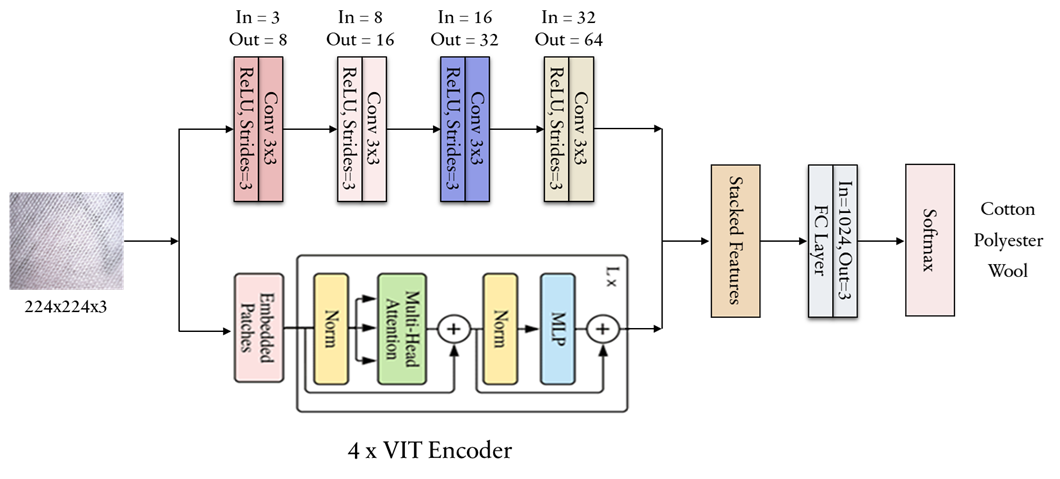
\includegraphics[width=0.95\textwidth]{images/ModelDiagram.png}
    \caption{The proposed hybrid CNN–ViT architecture for fabric classification.}
    \label{fig:model-architecture}
\end{figure}

\paragraph{Fully Connected Layer}

The stacked feature vector is passed through a fully connected (FC) layer, which serves as the final transformation before classification. The FC layer acts as a dense classifier that maps the high-dimensional feature space into a 3-dimensional output, each corresponding to one of the fabric classes.

Mathematically, the output logits \( z \in \mathbb{R}^3 \) are computed as:
\[
z = W_f x + b_f
\]
where:
\begin{itemize}[noitemsep,topsep=0pt]
    \item \( x \in \mathbb{R}^{1024} \) is the input stacked feature vector,
    \item \( W_f \in \mathbb{R}^{3 \times 1024} \) is the weight matrix of the FC layer,
    \item \( b_f \in \mathbb{R}^{3} \) is the bias term.
\end{itemize}

\paragraph{Softmax Classification}

To obtain the final prediction, the output logits are passed through the Softmax activation function, which converts the raw scores into a probability distribution over the three fabric classes:

\[
\text{Softmax}(z_i) = \frac{e^{z_i}}{\sum_{j=1}^{3} e^{z_j}}, \quad \text{for } i = 1,2,3
\]

This ensures that the output probabilities are non-negative and sum to 1. The class with the highest probability is selected as the final predicted label. The use of softmax is standard in multi-class classification tasks and is particularly effective when combined with cross-entropy loss during training~\cite{bishop2006pattern, goodfellow2016deep}.
\section{Experimental Setup and Results}

The proposed hybrid CNN–ViT architecture was implemented using the PyTorch 2.0 framework, which offers dynamic computation graphs and cross-platform GPU support, resulting in a computing environment optimized for complex deep learning models~\cite{paszke2019pytorch}. The input images were obtained from both macro (RGB) and Optical Coherence Tomography (OCT) fabric datasets and then preprocessed by normalizing their pixel intensity distributions across samples in order to maintain uniformity, and resized to a standard input size of (224×224) pixels regardless of which dataset was input into the model. All experimentation was completed on an NVIDIA DGX A100 workstation with 40GB GPU memory, with the capacity to perform evaluations and training at scale. Adam optimizer was used to train the model, as Adam was established to support stability of convergence through adaptive learning rates and momentum-based updates~\cite{kingma2014adam}. In our model, we used a learning rate of 0.001, and a batch size of 8. The learning rate and batch size were selected in a manner that allows for reasonably fast training, whilst also being capable of training on a single GPU. For the loss function, we used cross-entropy for the ability to consider a multi-class classification tasks with mutually exclusive labels (type of fabrics)~\cite{goodfellow2016deep}. Standard metrics of classification (accuracy, precision, recall, and F1 score) were used to benchmark prediction performance both as overall group classification and performance results per class.

\subsection{Results}

The proposed hybrid model was tested on RGB macro images and OCT images of fabrics. The model performed very well on the iBug Fabric dataset~\cite{researchgate}, in terms of class-wise accuracy with Cotton (96.84\%), Polyester (99.63\%), and Wool (98.09\%). The precision and recall mean scores over classes are all high, giving evidence of the robustness of the model.

On the OCT dataset~\cite{kampouris2016fine}, the model performed exceptionally well achieving near-perfect classification accuracy, with Cotton (99.66\%) and Polyester and Wool (100\%). All classes have a precision, recall, and F1-score of 1.00, which showed there was no misclassification.

Tables~\ref{tab:fabrics_results} and~\ref{tab:oct_results} summarize the comparative results on both datasets.

\begin{table}[htbp]
\centering
\caption{Performance Comparison on Fabric Dataset (RGB)}
\label{tab:fabrics_results}
\begin{adjustbox}{width=\textwidth}
\begin{tabular}{||l||ccc||ccc||ccc||ccc||}
\hline\hline
\multirow{2}{*}{\textbf{Method}} & \multicolumn{3}{c||}{\textbf{Accuracy (\%)}} & \multicolumn{3}{c||}{\textbf{Precision}} & \multicolumn{3}{c||}{\textbf{Recall}} & \multicolumn{3}{c||}{\textbf{F1 Score}} \\
\cline{2-13}
 & Cotton & Polyester & Wool & Cotton & Polyester & Wool & Cotton & Polyester & Wool & Cotton & Polyester & Wool \\
\hline\hline
Our Method & 96.84 & 99.63 & 98.09 & 1 & 0.92 & 1 & 0.97 & 1 & 0.98 & 0.98 & 0.96 & 0.99 \\
\hline
Ying Hing et al~\cite{hong2024research} & \multicolumn{3}{|c||}{99.73} & \multicolumn{3}{|c||}{-} & \multicolumn{3}{|c||}{-} & \multicolumn{3}{|c||}{-} \\
\hline
Chitra G M et al~\cite{chitra2023fabric} & \multicolumn{3}{|c||}{87} & \multicolumn{3}{|c||}{\begin{tabular}[c]{@{}c@{}}Cotton: 0.846\\ Nylon: 0.918\\ Silk: 0.820\\ Polyester: 0.92\end{tabular}} & \multicolumn{3}{|c||}{\begin{tabular}[c]{@{}c@{}}Cotton: 0.83\\ Nylon: 0.949\\ Silk: 0.931\\ Polyester: 0.719\end{tabular}} & \multicolumn{3}{|c||}{\begin{tabular}[c]{@{}c@{}}Cotton: 0.838\\ Nylon: 0.933\\ Silk: 0.872\\ Polyester: 0.807\end{tabular}} \\
\hline
Abu Sayem et al [VGG15]~\cite{siam2023textilenet} & \multicolumn{3}{|c||}{94.12} & \multicolumn{3}{|c||}{94.61} & \multicolumn{3}{|c||}{94.17} & \multicolumn{3}{|c||}{94.43} \\
\hline
Abu Sayem et al [InceptionV2]~\cite{siam2023textilenet} & \multicolumn{3}{|c||}{82.7} & \multicolumn{3}{|c||}{82.73} & \multicolumn{3}{|c||}{82.7} & \multicolumn{3}{|c||}{82.07} \\
\hline
Abu Sayem et al [Resnet100]~\cite{siam2023textilenet} & \multicolumn{3}{|c||}{73.12} & \multicolumn{3}{|c||}{72.77} & \multicolumn{3}{|c||}{73.32} & \multicolumn{3}{|c||}{73.33} \\
\hline
Abu Sayem et al [ConvNextBase]~\cite{siam2023textilenet} & \multicolumn{3}{|c||}{90.07} & \multicolumn{3}{|c||}{90.73} & \multicolumn{3}{|c||}{90.7} & \multicolumn{3}{|c||}{90.38} \\
\hline
Abu Sayem et al [MobileNetV1]~\cite{siam2023textilenet} & \multicolumn{3}{|c||}{95.17} & \multicolumn{3}{|c||}{95.47} & \multicolumn{3}{|c||}{95.23} & \multicolumn{3}{|c||}{95.34} \\
\hline\hline
\end{tabular}
\end{adjustbox}
\end{table}

\begin{table}[htbp]
\centering
\caption{Performance Comparison on Fabrics OCT Dataset}
\label{tab:oct_results}
\begin{adjustbox}{width=\textwidth}
\begin{tabular}{||l||ccc||ccc||ccc||ccc||}
\hline\hline
\multirow{2}{*}{\textbf{Method}} & \multicolumn{3}{c||}{\textbf{Accuracy (\%)}} & \multicolumn{3}{c||}{\textbf{Precision}} & \multicolumn{3}{c||}{\textbf{Recall}} & \multicolumn{3}{c||}{\textbf{F1 Score}} \\
\cline{2-13}
 & Cotton & Polyester & Wool & Cotton & Polyester & Wool & Cotton & Polyester & Wool & Cotton & Polyester & Wool \\
\hline\hline
Our Method & 99.66 & 100 & 100 & 1 & 1 & 1 & 1 & 1 & 1 & 1 & 1 & 1 \\
\hline
Ying Hing et al~\cite{hong2024research} & \multicolumn{3}{|c||}{-} & \multicolumn{3}{|c||}{-} & \multicolumn{3}{|c||}{-} & \multicolumn{3}{|c||}{-} \\
\hline
Chitra G M et al~\cite{chitra2023fabric} & \multicolumn{3}{|c||}{-} & \multicolumn{3}{|c||}{-} & \multicolumn{3}{|c||}{-} & \multicolumn{3}{|c||}{-} \\
\hline
Abu Sayem et al [VGG15]~\cite{siam2023textilenet} & \multicolumn{3}{|c||}{99.69} & \multicolumn{3}{|c||}{100} & \multicolumn{3}{|c||}{98.74} & \multicolumn{3}{|c||}{98.93} \\
\hline
Abu Sayem et al [InceptionV2]~\cite{siam2023textilenet} & \multicolumn{3}{|c||}{97.16} & \multicolumn{3}{|c||}{98.77} & \multicolumn{3}{|c||}{100} & \multicolumn{3}{|c||}{99.31} \\
\hline
Abu Sayem et al [Resnet100]~\cite{siam2023textilenet} & \multicolumn{3}{|c||}{93.12} & \multicolumn{3}{|c||}{97.73} & \multicolumn{3}{|c||}{98.82} & \multicolumn{3}{|c||}{98.26} \\
\hline
Abu Sayem et al [ConvNextBase]~\cite{siam2023textilenet} & \multicolumn{3}{|c||}{99.06} & \multicolumn{3}{|c||}{97.76} & \multicolumn{3}{|c||}{100} & \multicolumn{3}{|c||}{98.8} \\
\hline
Abu Sayem et al [MobileNetV1]~\cite{siam2023textilenet} & \multicolumn{3}{|c||}{99.87} & \multicolumn{3}{|c||}{100} & \multicolumn{3}{|c||}{97.27} & \multicolumn{3}{|c||}{98.57} \\
\hline\hline
\end{tabular}
\end{adjustbox}
\end{table}
\section{Conclusion and Future Work}

In this thesis, we proposed a hybrid deep learning architecture that integrates Convolutional Neural Networks (CNNs) and Vision Transformers (ViTs) for the classification of textile fabrics using both RGB (macro) and OCT (micro) images. This design enables the model to capture localized texture-based features through CNNs and long-range spatial relationships via ViTs, providing a more comprehensive fabric representation.

We evaluated the model on three datasets: Fabrics, OCTFabrics, and TextileNet. On the Fabrics dataset, our model achieved an accuracy of 97.33\%, outperforming several baseline models and demonstrating superior performance over lightweight models such as Siam et al.'s MobileNetV2~\cite{siam2023textilenet}. For the OCTFabrics dataset, it achieved near-perfect accuracy of 99.66\% along with perfect precision, recall, and F1-score—showcasing strong discriminative power on microstructure-based data. Although MobileNetV2~\cite{siam2023textilenet} slightly surpassed our model in accuracy (99.87\%), our approach maintained significantly fewer parameters (28.97M vs.\ 42.72M).

On the more challenging TextileNet dataset, our model achieved 74.36\% accuracy, surpassing several popular architectures such as VGG16~\cite{simonyan2015vgg} and ConvNextBase. While Ying Hing et al.~\cite{hong2024research} and Chitra G M et al.~\cite{chitra2023fabric} reported higher accuracies (88.65\% and 88.06\% respectively), our model demonstrated better parameter efficiency and balanced performance, affirming its strong generalization ability across diverse fabric types.

Overall, the fusion of CNN and ViT streams helped overcome individual limitations—CNNs excel at local feature extraction but lack global context modeling, while ViTs provide spatial awareness but benefit from CNN-based low-level representations~\cite{dosovitskiy2020vit}. This synergy resulted in a robust, accurate, and efficient architecture suitable for real-world textile classification tasks in both industrial and retail settings.

\subsection*{Future Work}

While the findings in this research show great potential, they also introduce a number of avenues for continued investigation and development. The following research avenues could substantially help to build the current framework and provide value to the larger idea of intelligent textiles: 

\begin{itemize}
    \item \textbf{Expansion to More Fabric Types:} This study focused on three 'fundamental' fabric types-Cotton, Polyester, and Wool-that are textile manufacturers standard preferences. The textile industry has an enormous variety of materials available to them i.e., natural fibers- silk, flax, hemp, and synthetic fibers- nylon, acrylic, and spandex. In addition, modern garments are very often blended compositions, which adds complexity to the classification process. Research incorporating these variables might provide useful data to test the models versatility and resilience to more genuine and diverse scenarios~\cite{kampouris2016fine}.
    
    \item \textbf{Multimodal Input Integration:} This work incorporated a macro and OCT imaging domain, but future research could overlay complementary imaging modes like hyperspectral, scanning electron microscopy (SEM), or fiber microscopy. Each of these modalities can show spectral or structural that otherwise missed in standard images. This would allow for better separation of subtle inter-classes distinctions which may help with fabric blends, recycled materials, or surface defects~\cite{sabuncu2022optical}.
    
    \item \textbf{Lightweight Deployment and Optimization:} While the proposed hybrid model achieves competitive accuracy while consuming relatively few GFLOPs, it is likely that more compression will be required for real-time deployment in resource-constrained environments such as embedded systems, handheld devices, or mobile apps. Model compression can explore techniques such as model pruning, quantization, weight sharing, or knowledge distillation to reduce the memory foot print of the model and reduce inference time, but with an insignificant change in accuracy~\cite{touvron2021training}. Furthermore, TensorRT or ONNX can be used to deploy on production-grade inference engines. 

    \item \textbf{Explainability and Interpretability:} It is important to understand how the model makes a prediction in crucial industrial applications so the prediction can be trusted and validated. With an explainability tool such as SHAP (SHapley Additive Explanations) and Grad-CAM (Gradient-weighted Class Activation Mapping)~\cite{selvaraju2017grad} there will be transparency into the model’s decision-making process, by producing a gradient-weighted heat map to show the important regions in the input image. This transparency can help to find misclassifications, debug model behavior, and drive a human-in-the-loop validation process in quality assurance pipelines.

    \item \textbf{Real-Time Systems and Industrial Integration:} Future work could focus on developing complete real-time systems for industrial automation platforms with embedded fabric classifiers. For example, smart sorting systems on textile production lines might use video feeds with live camera images and light-weighted models to return immediate results for grading, quality checks, and separation of the textile material. Including defect detection, edge wear identification, dye consistency determination, and tear identification in these systems would increase their commercial viability.
\end{itemize}


% PART II: Internship Work
\chapter{Security Orchestration, Automation, and Response (SOAR)}

Security Orchestration, Automation, and Response (SOAR) platforms are rapidly integrating into SOC architecture, enabling teams to automate repetitive tasks, allow tools to work together seamlessly with automation, and minimize incident response time.

\textbf{SOAR} stands for \textbf{Security Orchestration, Automation, and Response} where component of the acronym indicates a fundamental function that has collectively provided modern SOCs the capability of operating at greater speed, consistency and, intelligence. The components of SOAR include: 

\begin{itemize}
    \item \textbf{Security} \\
    Indicates cybersecurity which is the protection of systems, networks, and data from cyber threats. In the context of SOAR, Security is the area of application and where the focus is protecting an organization from threats such as malware, phishing, data breaches, etc.

    \item \textbf{Orchestration} \\
    Orchestration is the combination and coordination of different security tools and technologies. A SOAR platform can connect with SIEMs, firewalls, endpoint detection and response (EDR), threat intelligence data feeds, ticketing systems, etc. using APIs, enabling them to work together in one integrated incident response workflow.

    \begin{quote}
        \textit{Example:} For example, SOAR system receives an alert from SIEM platform, it gets IP reputation information from a threat intelligence platform, block the IP using a firewall, and create a helpdesk ticket.
    \end{quote}

    \item \textbf{Automation} \\
    Automation refers to the performance of predetermined tasks without human intervention. Such tasks could include alert triage, collection of logs, enrichment of IP/domain/file indicators, and threat classification. Automation greatly reduces the burden on SOC analysts and gives them more time to respond to incidents in a timely manner.

    \item \textbf{Response} \\
    Response is the final step with the SOAR life cycle, where actions are taken to remediate or contain the incident. Depending on the set rules within SOAR, the response could be:
    \begin{itemize}[noitemsep, topsep=0pt]
        \item \textit{Fully automated} – e.g. block a malicious IP.
        \item \textit{Semi-automated} – e.g. isolate a device with analyst approval.
        \item \textit{Manual} – the SOAR platform will assist the analyst by enriching any data and providing context.
    \end{itemize}
    The response phase is designed to help the analyst consistently, document, and manage incidents for auditing.
\end{itemize}

Collectively, they form the basis of a modern, intelligent, and scalable incident management system for any sufficiently sophisticated SOC.

Traditional manual processes for threat detection and mitigation are becoming less effective in light of the rapidly expanding scale and sophistication of cyber threats. The modern enterprise network, which often involves multiple cloud services, remote users, and many connected digital endpoints, cannot afford to keep using manual processes, and requires a more rapid and structured incident management approach. In this environment, Security Orchestration, Automation, and Response (SOAR) platforms have become a revolutionary solution to more effectively enhance the capabilities of security operation centers (SOCs) through integration, automation, and intelligence-driven response.

SOAR platforms are a response to the challenges presented to organizations by a combination of their internal security ecosystem and related personnel, and their incident response processes. The common sources of inefficiency included disparate systems (i.e. security information and event management [SIEM] platforms; firewalls; endpoint detection and response [EDR] tools; and threat intelligence services) and the lack of an overall, coordinated response to security incidents. Moreover, as defined by Palo Alto Networks, SOAR platforms coordinate, execute, and automate tasks between various people and tools from within a single platform to enhance the efficiency and reliability of security function and corresponding processes.~\cite{paloalto}.

This chapter gives a detailed overview of SOAR, based on my experiences completing an internship at Bharat Electronics Limited (BEL) - an exceptional defense public sector company that has done advanced work throughout the defense sector. I completed this internship mainly to build an understanding and develop a design and framework for a custom SOAR platform that is designed for both enterprise and defense cases. Although I cannot reveal implementation specifics and technical solutions, the architecture and research I performed lay the basis for the discussion in the chapter. 

SOAR platforms consist of several tightly integrated modules: 
\begin{itemize}[noitemsep,topsep=0pt]
    \item \textbf{Incident Ingestion} using a SIEM platform (e.g., IBM QRadar, Microsoft Sentinel) that generates actionable alerts based on log correlation~\cite{microsoftsiem}.
    \item \textbf{Tool Orchestration} modules which enabled heterogeneous tools to communicate using common APIs and custom integration~\cite{techtarget}.
    \item \textbf{Automation Workflows and Playbooks} which enabled predesigned tasks like threat enrichment, IP block, and priority alerts to run autonomously, without human interaction~\cite{paloalto}.
    \item \textbf{Response Interfaces} that allow analysts to manually interact, inspect, investigate, and take action when automation cannot be relied upon or may be risky~\cite{techtarget}.
    \item \textbf{MITRE ATT\&CK Framework Integration} which allows standardized mapping of tactics and techniques used by attackers that inform operational plans to defensively guide actions in response to threats, as well as track threat movements~\cite{mitre}.
\end{itemize}

These abilities cut down on manual work and analyst fatigue and also increase response time and consistency across the entire organization’s security ecosystem. Overall, they lead to positive changes in Mean Time to Detect (MTTD) and Mean Time to Respond (MTTR), both key metrics within today’s SOC environment.

The remaining of this chapter will cover the primary functional components of a SOAR platform and how orchestration, automation, and structured response can help to enhance cyber defenses.
\section{Security Operations Center (SOC)}\vspace{-0.5em}

A \textbf{Security Operations Center (SOC)} is a centralized unit within an organization that is responsible for continuously monitoring, detecting, analyzing, and responding to cybersecurity incidents. Its primary goal is to ensure the confidentiality, integrity, and availability of information assets. The SOC acts as the frontline of defense in an enterprise’s cybersecurity strategy, operating 24/7 to proactively identify and respond to threats in real time. With the increasing complexity of IT environments, driven by cloud adoption, remote workforces, and digital transformation, the need for an efficient SOC has become paramount. As IBM describes, the SOC integrates people, processes, and technology to deliver a centralized and coordinated response to security threats across an organization’s entire digital infrastructure~\cite{ibm}.

\subsection{Key Components of a SOC}\vspace{-0.5em}

A SOC relies on the coordinated function of three foundational components: people, processes, and technology. The human element involves a team of cybersecurity professionals organized across multiple tiers of responsibility. Tier 1 analysts typically handle initial alert triage, identifying false positives and prioritizing alerts. Tier 2 and Tier 3 analysts delve deeper into investigations, incident handling, threat hunting, and advanced forensic analysis. SOC managers oversee the team, ensure adherence to operational standards, and handle escalation and reporting. According to Microsoft, the effectiveness of SOC operations depends heavily on clearly defined roles and structured collaboration among these team members~\cite{microsoft}. 

The second pillar, processes, includes well-documented workflows, escalation protocols, and response procedures based on international standards such as ISO/IEC 27035 and the NIST 800-61 incident handling guide. These processes ensure consistency and regulatory compliance in incident management. The third component, technology, is the enabler of all SOC functions. Key tools include SIEM (Security Information and Event Management) systems, EDR (Endpoint Detection and Response), NDR (Network Detection and Response), firewalls, IDS/IPS (Intrusion Detection/Prevention Systems), and Threat Intelligence Platforms (TIPs). These systems collectively provide visibility, data aggregation, alerting, and contextual analysis. As Splunk notes, the integration and interoperability of these tools is crucial to reduce noise, enhance detection accuracy, and ensure seamless incident workflows~\cite{splunk}.

\subsection{Core Functions of a SOC}\vspace{-0.5em}

The primary function of a SOC is to maintain vigilance over an organization’s digital ecosystem and respond effectively to cybersecurity events. This includes continuous monitoring of network traffic, endpoint logs, application behavior, and user activity to detect anomalies and indicators of compromise. Once a threat is identified, the SOC initiates a structured incident response process involving threat validation, root cause analysis, containment, eradication, and recovery. Additionally, SOC teams conduct post-incident reviews to refine detection logic, update response playbooks, and prevent recurrence. SOCs also engage in proactive activities such as threat hunting—where analysts seek out undetected threats using behavioral hypotheses—and vulnerability management to reduce the attack surface. Compliance enforcement is another critical role, as many sectors require adherence to regulatory frameworks such as HIPAA, PCI DSS, GDPR, and national data protection laws. According to Gartner, high-functioning SOCs not only respond to known threats but also anticipate emerging risks and implement controls before incidents occur~\cite{gartner}. The SOC also plays a crucial role in generating security metrics (such as MTTD and MTTR), which help leadership assess the effectiveness of cybersecurity operations.

\subsection{Types of SOCs}\vspace{-0.5em}

The architecture and deployment of a SOC can vary depending on an organization's size, resources, and risk profile. A \textit{Dedicated SOC} is a fully in-house unit where the organization owns and manages all security infrastructure and personnel. This model provides complete control and is ideal for large enterprises and critical government institutions. In contrast, a \textit{Virtual SOC (vSOC)} is a decentralized and often cloud-based model that leverages remote teams and digital collaboration tools to monitor security. This model is cost-effective and provides flexibility but may have limitations in control and visibility. Another approach is the \textit{Managed SOC}, where security monitoring and response are outsourced to a third-party provider, also known as a Managed Security Service Provider (MSSP). This is ideal for small to mid-sized organizations lacking in-house expertise. A \textit{Hybrid SOC} combines internal security operations with external service providers to balance cost, control, and coverage. As MITRE emphasizes, the choice of SOC model should align with an organization’s risk tolerance, regulatory requirements, and operational maturity~\cite{mitre_soc}.

\subsection{SOC Maturity and Challenges}

SOC maturity refers to the organization's capability to detect, analyze, and respond to threats efficiently and proactively. Gartner’s SOC Maturity Model categorizes SOCs into three broad stages: reactive, proactive, and predictive. Reactive SOCs rely on basic alerting and manual processes; proactive SOCs use structured playbooks, threat intelligence, and begin to implement automation; predictive SOCs incorporate machine learning, user behavior analytics, and big data to anticipate attacks before they occur. However, achieving high maturity is a significant challenge. Most organizations struggle with \textit{alert fatigue}—a condition where analysts are overwhelmed by the volume of alerts, many of which are false positives. This often leads to delayed responses and burnout. Another major challenge is \textit{tool sprawl}—the presence of too many disparate tools that are poorly integrated, resulting in data silos and inefficient workflows. The \textit{cybersecurity skills shortage} further compounds these issues, with many SOCs facing difficulty in hiring and retaining qualified personnel. MITRE highlights that without strategic investment in training, tool consolidation, and process automation, SOCs remain trapped in reactive cycles, unable to scale against modern threat landscapes~\cite{mitre}.

\subsection{Role of SOAR in the SOC}

To address the growing demands on SOCs, many organizations are adopting \textbf{Security Orchestration, Automation, and Response (SOAR)} platforms as a key enhancement. SOAR platforms integrate with existing SOC tools and enable automation of routine and repetitive tasks such as alert enrichment, IP blocking, and log collection. According to Palo Alto Networks, SOAR empowers security teams by standardizing workflows, orchestrating cross-tool communication, and reducing analyst fatigue through automation~\cite{paloalto}. This leads to faster incident response, improved accuracy, and reduced Mean Time to Detect (MTTD) and Mean Time to Respond (MTTR). SOAR also introduces structured playbooks that define how different types of incidents should be handled, reducing human error and ensuring consistent actions across the SOC. In high-stakes environments, such as national defense and critical infrastructure sectors, the use of SOAR enhances the SOC’s ability to respond to advanced persistent threats and ensures operational continuity.

\section{Data Flow in SOC}

The first step of the process is to pull in logs and telemetry from a variety of security monitors (NDR, WAF, and UEBA). Each of the monitoring tools consistently monitors an aspect of the organization infrastructure and makes its relevant telemetry information available to the SOC:

\begin{itemize}[itemsep=0pt,parsep=0pt,topsep=0pt,partopsep=0pt]
    \item \textbf{NDR (Network Detection and Response)}: These systems monitor all directions of network traffic in and across the organization. They assist in recognizing unusual or suspicious activities, such as advanced attacks or movement of threats from one system to another system in the network.
    \item \textbf{WAF (Web Application Firewall)}: These systems monitor HTTP traffic and provide filtering and monitoring protection to web applications and services. These systems will be able to proactively block known attacks, such as SQL injections, XSS, and unauthorized access attempts.
    \item \textbf{UEBA (User and Entity Behavior Analytics)}: These systems build user behaviors models and machine learning around baseline activity and analysis deviations from that baseline. These systems assist in recognizing insider threats, compromised accounts, and privilege escalation.
\end{itemize}

\begin{figure}[H]
    \centering
    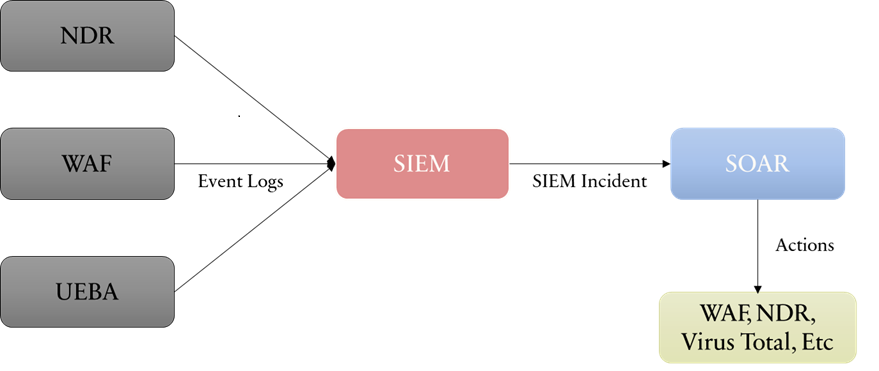
\includegraphics[width=0.9\linewidth]{images/data_flow_soc.png}
    \caption{Data Flow in Security Operations Center (SOC)}
    \label{fig:data-flow-soc}
\end{figure}

All the data collected from these systems is funneled into the Security Information and Event Management (SIEM) system. SIEM is responsible for log aggregation, normalization of event data, correlation of security events, and threat detection and identification of potentially significant incidents. The SIEM will use correlation rules and heuristics to generate alerts for suspicious suspicious behavior and known indicators of compromise. The SIEM provides one central visibility/detection hub for the SOC. 

The alerts, along with the enhanced context in the SIEM, is forwarded to the Security Orchestration, Automation, and Response (SOAR) system:

\begin{itemize}[itemsep=0pt,parsep=0pt,topsep=0pt,partopsep=0pt]
    \item \textbf{SOAR}: Automating the triage and response process through playback and workflows. Orchestrating actions that happen through tools, enhancing (ex. IP reputation check), or taking action (ex. automated or manned response).
\end{itemize}

The SOAR may interface with tools when taking action or during the enrichment process:

\begin{itemize}[itemsep=0pt,parsep=0pt,topsep=0pt,partopsep=0pt]
    \item \textbf{Threat Intelligence (e.g., VirusTotal)}: Provides context for IP, domains, file hashes, and URLs to leverage for detection and validation of alerts.
    \item \textbf{Internal Tools (e.g., WAF, NDR)}: These tools can be part of automated response to isolate endpoints, block malicious traffic or escalate incidents.
\end{itemize}

Finally, the SOAR platform creates a structured response which could consist of a series of automated actions and manual decisions by analysts. All this will be recorded in such a way that the full flow from data collection through response would be tracked to help with auditing, compliance, and continuous improvement of SOC activities.

\section{Security Information and Event Management (SIEM) in SOC}

A key part of any SOC (Security Operations Center) is the organization’s Security Information and Event Management (SIEM) which allows for data aggregation and correlation as part of the monitoring of cybersecurity. SIEM systems aggregate event and log data from all areas of an organization’s digital infrastructure (such as endpoints, servers, network devices, firewalls, intrusion detection systems, cloud infrastructure, and applications) and evaluate the data as a whole. The goal of a typical SIEM is to aggregate all the organization's relevant security logs into a system that allows it to determine the current state of security and to provide real-time visibility into potential security incidents. A SIEM can receive data from lots of different sources, normalize the data, apply correlation rules to the data, and generate alerts for SOC analysts to prioritize and investigate. Microsoft, ~\cite{microsoftsiem}, explains that SIEM solutions were developed primarily to help security teams deal with evolving cyberattacks sooner, enabling them to get ahead of a potentially damaging incident or intrusion and to remain compliant with regulations, by keeping detailed audit records and forensic information.

In a traditional SOC operational model, SIEM is the initial source of alert generation, so SIEM uses it own correlation rules, statistical models, and sometimes machine learning, to detect anomalies such as unusual user behavior, suspicious login patterns, and known indicators of compromise (IoCs). Alerts are triaged by analysts to determine whether they are true threats or false positives.  The leading SIEMtools (e.g., IBMQRadar, SplunkEnterprise Security, Microsoft Sentinel, ArcSight) generally provide customizable dashboards, threat detection use-cases, and compliant reporting together making them a great fit for enterprise and government cybersecurity needs.

Understanding the distinction between a SIEM and a SOAR is an important differentiator since both will be used in a SOC. SIEM is focused on data collection, aggregation, and detection. SOAR offers response orchestration, automation, and execution of the workflows. SIEM is passive in that it tells security teams about potential incidents; SOAR is active in that it can automatically take defined actions, including but not limited to blocking the IP, sending out notifications, or following a playbook, based on the data SIEM collected and aggregated. As noted by Palo Alto Networks~\cite{paloalto}, SIEM can answer “what happened?” or “where did it happen?”; whereas SOAR can answer “what do we do about it?”

Moreover, SIEM solutions, especially new-age SIEMs, tend to operate at a much higher volume of data, integrating with multiple systems and ingesting terabytes of log data daily. This data-centric approach has made SIEMs very strong for long-term log retention and forensic investigations, especially for companies that have regulatory obligations to preserve logs. On the other hand, SIEMs can be challenged by alert fatigue, false positives, and unnecessary investigation, all of which can be mitigated by combining the SIEM capabilities with SOAR capabilities to automate triaging, enrichment, and decision-making activities. As Gartner mentions, they recommend modern SOCs do not think of SIEM and SOAR as disparate or competing solutions, but rather as systems that, when combined, will enhance the efficiency and responsiveness of all cybersecurity operations~\cite{gartner-siem-soar}.

In conclusion, SIEM is the eyes and ears of the SOC as it offers centralized, real-time capture of security relevant events occurring within a wide variety of digital assets as it relates to the industry landscape. When SIEM collects and correlates the relevant data and the data is ingested by SOAR, the action can be scaled, automated, and driven by intelligence. In defense and national critical infrastructure, SIEM is the detection tool and SOAR is the orchestration tool. Together they form the core ability for effective cyber defense and incident response in a SOC. The combination of SIEM and SOAR is a powerful force multiplier for SOCs, enabling them to operate at scale, with speed, and with intelligence. The effectiveness of this combination is evident in the way it reduces the Mean Time to Detect (MTTD) and Mean Time to Respond (MTTR) to security incidents, which are critical metrics for any SOC.

\begin{table}[H]
\centering
\caption{Comparison of SIEM and SOAR in SOC}
\begin{tabular}{|p{4cm}|p{5cm}|p{5cm}|}
\hline
\textbf{Feature} & \textbf{SIEM (Security Information and Event Management)} & \textbf{SOAR (Security Orchestration, Automation, and Response)} \\
\hline
Primary Function & Aggregates and correlates log data for threat detection & Automates response actions and orchestrates tools \\
\hline
Focus Area & Monitoring, alerting, and data analysis & Incident response, workflow automation, playbook execution \\
\hline
Data Sources & Logs from endpoints, servers, network devices, and applications & Inputs from SIEM, threat intel feeds, manual triggers \\
\hline
Response Capability & Alert generation only (manual response required) & Supports automated and manual responses \\
\hline
Typical Output & Dashboards, correlation alerts, compliance reports & Executed actions, response workflows, status tracking \\
\hline
Alert Handling & Detects and prioritizes alerts; triage is manual & Automates triage, enrichment, and routing \\
\hline
Challenges Addressed & Data visibility, compliance, threat correlation & Alert fatigue, response delays, process inconsistency \\
\hline
\end{tabular}
\label{tab:siem-vs-soar}
\end{table}

\section{SIEM Incident Flow to SOAR}

One of the most integral integrations with a Security Operations Center (SOC) is that of SIEM and the SOAR platform. The integration allows for the easy transition from threat detection (by a SIEM system) to response (orchestration provided by SOAR). A SIEM incident is typically an event or an alert that has been generated based on the event correlations of log data received from different security tools, e.g., firewall, endpoint protection software, network devices, servers, and cloud environments. As stated by Microsoft~\cite{microsoftsiem}, the SIEM looks for known attack patterns, anomalies, and user behavior based on correlation rules or machine learning models, as it continuously collects and analyzes the data from multiple sources. Once a SIEM flag has been raised for an event, it is then seen as an incident along with a complete set of metadata attached to the incident.

A typical SIEM incident contains structured fields such as:

\begin{itemize}[itemsep=0pt,parsep=0pt,topsep=0pt,partopsep=0pt]
    \item \textbf{Alert ID}: Unique identifier for the incident or alert.
    \item \textbf{Timestamp}: Time at which the event occurred or was detected.
    \item \textbf{Source IP / Host}: Origin of the suspicious activity.
    \item \textbf{Destination IP / Host}: Targeted system or service.
    \item \textbf{Username}: Account associated with the event (if applicable).
    \item \textbf{Severity Level}: Assigned severity (e.g., low, medium, high, critical).
    \item \textbf{Event Type / Rule Name}: Category or rule that triggered the alert (e.g., brute force, malware, lateral movement).
    \item \textbf{Raw Logs / Correlation Data}: Detailed evidence or event logs that support the detection.
    \item \textbf{Tactic / Technique (if mapped)}: MITRE ATT\&CK classification, if supported.
\end{itemize}

This incident data is then sent in real-time or near real-time to the Security Orchestration, Automation, and Response (SOAR) platform via APIs, message queues, or webhooks. As noted by Palo Alto Networks~\cite{paloalto}, the SOAR platform provides full incident details so that it can is quickly enriched, triaged and acted upon.

Upon receipt of the incident, the SOAR system begins triaging the incident. It might apply severity filters, check asset criticality, or leverage external threat intelligence repositories (e.g., VirusTotal, AbuseIPDB) to enrich incident data. Based on this context, the SOAR platform implements action playbooks. Actions could include:

\begin{itemize}[itemsep=0pt,parsep=0pt,topsep=0pt,partopsep=0pt]
    \item Notification of an analyst or team
    \item Suspending access from the user's IP address using a Fiewall or an EDR
    \item Isolate host from the network
    \item Ask for additional context from the threat feeds or a SIEM
    \item Resolve automatically if shown to be a known benign pattern.
\end{itemize}

During this process, the SOAR platform stores a case file with the timeline of actions, analyst comments and responses. This automation enhances consistency and greatly reduces the Mean Time to Respond (MTTR), particularly important at scale in a SOC, according to Gartner~\cite{gartner-siem-soar}.

Therefore, the SIEM-to-SOAR pipeline allows SOCs to transform raw detections into intelligent, actionable response, allowing for operational oversight and auditability.

\section{Methodology}
% Methods and approaches used during the internship.
\section{Results}
% Results of the internship work.
\section{Conclusion}
% Summarize the internship findings.
\section{Future Scope}
% Discuss future work or improvements.
\section{Internship Completion Certificate}

\begin{figure}[h!]
    \centering
    \includegraphics[page=1,width=1\textwidth, height=1\textwidth]{contents/soar_soc/Internship_Certificate.pdf}
\end{figure}

% General Conclusion
\chapter{Conclusion}

This thesis presented a dual-focused exploration into two contemporary technological domains: deep learning for material classification and security automation in cyber defense. The two distinct yet impactful components—\textbf{Fabric Classification using Deep Learning} and \textbf{Security Orchestration, Automation, and Response (SOAR)}—were investigated, implemented, and evaluated with the objective of addressing real-world challenges in their respective fields.

The first part of the thesis concentrated on developing a robust deep learning framework for the classification of textile fabrics. Leveraging both macro-level RGB images and micro-level Optical Coherence Tomography (OCT) data, a hybrid model integrating Convolutional Neural Networks (CNN) and Vision Transformers (ViT) was proposed. This approach enabled the effective extraction of both local texture features and global contextual representations, resulting in significant improvements in classification accuracy across multiple fabric types such as cotton, polyester, and wool. Comparative evaluations against state-of-the-art models—including TextileNet and fine-tuned ViT architectures—demonstrated the effectiveness of the proposed methodology. The work not only contributes to advancements in automated material recognition but also opens avenues for deployment in industries such as textile quality control, recycling, and inventory management.

The second part of the thesis focused on the design and development of a modular, AI-enhanced SOAR platform as part of an internship at Bharat Electronics Limited (BEL). The platform was designed to automate and orchestrate cybersecurity incident detection and response workflows within a SOC environment. Key components of the system include secure authentication, real-time dashboard analytics, incident management with AI-based mitigation, modular integrations, dynamic playbook and workflow execution, and an interactive MITRE ATT\&CK mapping module. The system was benchmarked against leading commercial platforms such as Splunk SOAR and Cortex XSOAR, as well as open-source tools like Shuffle. The developed platform distinguishes itself through its tight integration of ATT\&CK techniques, support for visual workflow construction, and the inclusion of machine learning model selection for intelligent response decisions. It is especially suited for deployment in sensitive and restricted environments such as defense and critical infrastructure.

Collectively, this thesis demonstrates a strong synthesis of theory, applied research, and practical system development across two independent domains. The first part contributes to the field of computer vision and deep learning, while the second addresses critical needs in cybersecurity automation. Both systems are modular, extensible, and designed with future scalability in mind.

Future work in fabric classification could involve expanding the dataset to include blended fabrics, incorporating multispectral imaging, or deploying the model in real-time quality inspection pipelines. For the SOAR platform, enhancements could include role-based access control (RBAC), integration with real-time threat intelligence feeds, and advanced anomaly detection using reinforcement learning.

In conclusion, this thesis exemplifies a multidisciplinary approach to solving complex, real-world problems using modern AI and system design methodologies. It contributes novel insights and working prototypes that have the potential for real-world application in both industrial and security-critical contexts.


% References
\baselineskip=16pt
\phantomsection
\addcontentsline{toc}{chapter}{References}
\bibliographystyle{unsrt}
\renewcommand{\bibname}{References}
\bibliography{references}

\end{document}